\documentclass[11pt]{article}

    \usepackage[breakable]{tcolorbox}
    \usepackage{parskip} % Stop auto-indenting (to mimic markdown behaviour)
    
    \usepackage{iftex}
    \ifPDFTeX
    	\usepackage[T1]{fontenc}
    	\usepackage{mathpazo}
    \else
    	\usepackage{fontspec}
    \fi

    % Basic figure setup, for now with no caption control since it's done
    % automatically by Pandoc (which extracts ![](path) syntax from Markdown).
    \usepackage{graphicx}
    % Maintain compatibility with old templates. Remove in nbconvert 6.0
    \let\Oldincludegraphics\includegraphics
    % Ensure that by default, figures have no caption (until we provide a
    % proper Figure object with a Caption API and a way to capture that
    % in the conversion process - todo).
    \usepackage{caption}
    \DeclareCaptionFormat{nocaption}{}
    \captionsetup{format=nocaption,aboveskip=0pt,belowskip=0pt}

    \usepackage{float}
    \floatplacement{figure}{H} % forces figures to be placed at the correct location
    \usepackage{xcolor} % Allow colors to be defined
    \usepackage{enumerate} % Needed for markdown enumerations to work
    \usepackage{geometry} % Used to adjust the document margins
    \usepackage{amsmath} % Equations
    \usepackage{amssymb} % Equations
    \usepackage{textcomp} % defines textquotesingle
    % Hack from http://tex.stackexchange.com/a/47451/13684:
    \AtBeginDocument{%
        \def\PYZsq{\textquotesingle}% Upright quotes in Pygmentized code
    }
    \usepackage{upquote} % Upright quotes for verbatim code
    \usepackage{eurosym} % defines \euro
    \usepackage[mathletters]{ucs} % Extended unicode (utf-8) support
    \usepackage{fancyvrb} % verbatim replacement that allows latex
    \usepackage{grffile} % extends the file name processing of package graphics 
                         % to support a larger range
    \makeatletter % fix for old versions of grffile with XeLaTeX
    \@ifpackagelater{grffile}{2019/11/01}
    {
      % Do nothing on new versions
    }
    {
      \def\Gread@@xetex#1{%
        \IfFileExists{"\Gin@base".bb}%
        {\Gread@eps{\Gin@base.bb}}%
        {\Gread@@xetex@aux#1}%
      }
    }
    \makeatother
    \usepackage[Export]{adjustbox} % Used to constrain images to a maximum size
    \adjustboxset{max size={0.9\linewidth}{0.9\paperheight}}

    % The hyperref package gives us a pdf with properly built
    % internal navigation ('pdf bookmarks' for the table of contents,
    % internal cross-reference links, web links for URLs, etc.)
    \usepackage{hyperref}
    % The default LaTeX title has an obnoxious amount of whitespace. By default,
    % titling removes some of it. It also provides customization options.
    \usepackage{titling}
    \usepackage{longtable} % longtable support required by pandoc >1.10
    \usepackage{booktabs}  % table support for pandoc > 1.12.2
    \usepackage[inline]{enumitem} % IRkernel/repr support (it uses the enumerate* environment)
    \usepackage[normalem]{ulem} % ulem is needed to support strikethroughs (\sout)
                                % normalem makes italics be italics, not underlines
    \usepackage{mathrsfs}
    

    
    % Colors for the hyperref package
    \definecolor{urlcolor}{rgb}{0,.145,.698}
    \definecolor{linkcolor}{rgb}{.71,0.21,0.01}
    \definecolor{citecolor}{rgb}{.12,.54,.11}

    % ANSI colors
    \definecolor{ansi-black}{HTML}{3E424D}
    \definecolor{ansi-black-intense}{HTML}{282C36}
    \definecolor{ansi-red}{HTML}{E75C58}
    \definecolor{ansi-red-intense}{HTML}{B22B31}
    \definecolor{ansi-green}{HTML}{00A250}
    \definecolor{ansi-green-intense}{HTML}{007427}
    \definecolor{ansi-yellow}{HTML}{DDB62B}
    \definecolor{ansi-yellow-intense}{HTML}{B27D12}
    \definecolor{ansi-blue}{HTML}{208FFB}
    \definecolor{ansi-blue-intense}{HTML}{0065CA}
    \definecolor{ansi-magenta}{HTML}{D160C4}
    \definecolor{ansi-magenta-intense}{HTML}{A03196}
    \definecolor{ansi-cyan}{HTML}{60C6C8}
    \definecolor{ansi-cyan-intense}{HTML}{258F8F}
    \definecolor{ansi-white}{HTML}{C5C1B4}
    \definecolor{ansi-white-intense}{HTML}{A1A6B2}
    \definecolor{ansi-default-inverse-fg}{HTML}{FFFFFF}
    \definecolor{ansi-default-inverse-bg}{HTML}{000000}

    % common color for the border for error outputs.
    \definecolor{outerrorbackground}{HTML}{FFDFDF}

    % commands and environments needed by pandoc snippets
    % extracted from the output of `pandoc -s`
    \providecommand{\tightlist}{%
      \setlength{\itemsep}{0pt}\setlength{\parskip}{0pt}}
    \DefineVerbatimEnvironment{Highlighting}{Verbatim}{commandchars=\\\{\}}
    % Add ',fontsize=\small' for more characters per line
    \newenvironment{Shaded}{}{}
    \newcommand{\KeywordTok}[1]{\textcolor[rgb]{0.00,0.44,0.13}{\textbf{{#1}}}}
    \newcommand{\DataTypeTok}[1]{\textcolor[rgb]{0.56,0.13,0.00}{{#1}}}
    \newcommand{\DecValTok}[1]{\textcolor[rgb]{0.25,0.63,0.44}{{#1}}}
    \newcommand{\BaseNTok}[1]{\textcolor[rgb]{0.25,0.63,0.44}{{#1}}}
    \newcommand{\FloatTok}[1]{\textcolor[rgb]{0.25,0.63,0.44}{{#1}}}
    \newcommand{\CharTok}[1]{\textcolor[rgb]{0.25,0.44,0.63}{{#1}}}
    \newcommand{\StringTok}[1]{\textcolor[rgb]{0.25,0.44,0.63}{{#1}}}
    \newcommand{\CommentTok}[1]{\textcolor[rgb]{0.38,0.63,0.69}{\textit{{#1}}}}
    \newcommand{\OtherTok}[1]{\textcolor[rgb]{0.00,0.44,0.13}{{#1}}}
    \newcommand{\AlertTok}[1]{\textcolor[rgb]{1.00,0.00,0.00}{\textbf{{#1}}}}
    \newcommand{\FunctionTok}[1]{\textcolor[rgb]{0.02,0.16,0.49}{{#1}}}
    \newcommand{\RegionMarkerTok}[1]{{#1}}
    \newcommand{\ErrorTok}[1]{\textcolor[rgb]{1.00,0.00,0.00}{\textbf{{#1}}}}
    \newcommand{\NormalTok}[1]{{#1}}
    
    % Additional commands for more recent versions of Pandoc
    \newcommand{\ConstantTok}[1]{\textcolor[rgb]{0.53,0.00,0.00}{{#1}}}
    \newcommand{\SpecialCharTok}[1]{\textcolor[rgb]{0.25,0.44,0.63}{{#1}}}
    \newcommand{\VerbatimStringTok}[1]{\textcolor[rgb]{0.25,0.44,0.63}{{#1}}}
    \newcommand{\SpecialStringTok}[1]{\textcolor[rgb]{0.73,0.40,0.53}{{#1}}}
    \newcommand{\ImportTok}[1]{{#1}}
    \newcommand{\DocumentationTok}[1]{\textcolor[rgb]{0.73,0.13,0.13}{\textit{{#1}}}}
    \newcommand{\AnnotationTok}[1]{\textcolor[rgb]{0.38,0.63,0.69}{\textbf{\textit{{#1}}}}}
    \newcommand{\CommentVarTok}[1]{\textcolor[rgb]{0.38,0.63,0.69}{\textbf{\textit{{#1}}}}}
    \newcommand{\VariableTok}[1]{\textcolor[rgb]{0.10,0.09,0.49}{{#1}}}
    \newcommand{\ControlFlowTok}[1]{\textcolor[rgb]{0.00,0.44,0.13}{\textbf{{#1}}}}
    \newcommand{\OperatorTok}[1]{\textcolor[rgb]{0.40,0.40,0.40}{{#1}}}
    \newcommand{\BuiltInTok}[1]{{#1}}
    \newcommand{\ExtensionTok}[1]{{#1}}
    \newcommand{\PreprocessorTok}[1]{\textcolor[rgb]{0.74,0.48,0.00}{{#1}}}
    \newcommand{\AttributeTok}[1]{\textcolor[rgb]{0.49,0.56,0.16}{{#1}}}
    \newcommand{\InformationTok}[1]{\textcolor[rgb]{0.38,0.63,0.69}{\textbf{\textit{{#1}}}}}
    \newcommand{\WarningTok}[1]{\textcolor[rgb]{0.38,0.63,0.69}{\textbf{\textit{{#1}}}}}
    
    
    % Define a nice break command that doesn't care if a line doesn't already
    % exist.
    \def\br{\hspace*{\fill} \\* }
    % Math Jax compatibility definitions
    \def\gt{>}
    \def\lt{<}
    \let\Oldtex\TeX
    \let\Oldlatex\LaTeX
    \renewcommand{\TeX}{\textrm{\Oldtex}}
    \renewcommand{\LaTeX}{\textrm{\Oldlatex}}
    % Document parameters
    % Document title
    \title{Remarks on COVID-19 Dynamics in Switzerland}
    
    
    
    
    
% Pygments definitions
\makeatletter
\def\PY@reset{\let\PY@it=\relax \let\PY@bf=\relax%
    \let\PY@ul=\relax \let\PY@tc=\relax%
    \let\PY@bc=\relax \let\PY@ff=\relax}
\def\PY@tok#1{\csname PY@tok@#1\endcsname}
\def\PY@toks#1+{\ifx\relax#1\empty\else%
    \PY@tok{#1}\expandafter\PY@toks\fi}
\def\PY@do#1{\PY@bc{\PY@tc{\PY@ul{%
    \PY@it{\PY@bf{\PY@ff{#1}}}}}}}
\def\PY#1#2{\PY@reset\PY@toks#1+\relax+\PY@do{#2}}

\expandafter\def\csname PY@tok@w\endcsname{\def\PY@tc##1{\textcolor[rgb]{0.73,0.73,0.73}{##1}}}
\expandafter\def\csname PY@tok@c\endcsname{\let\PY@it=\textit\def\PY@tc##1{\textcolor[rgb]{0.25,0.50,0.50}{##1}}}
\expandafter\def\csname PY@tok@cp\endcsname{\def\PY@tc##1{\textcolor[rgb]{0.74,0.48,0.00}{##1}}}
\expandafter\def\csname PY@tok@k\endcsname{\let\PY@bf=\textbf\def\PY@tc##1{\textcolor[rgb]{0.00,0.50,0.00}{##1}}}
\expandafter\def\csname PY@tok@kp\endcsname{\def\PY@tc##1{\textcolor[rgb]{0.00,0.50,0.00}{##1}}}
\expandafter\def\csname PY@tok@kt\endcsname{\def\PY@tc##1{\textcolor[rgb]{0.69,0.00,0.25}{##1}}}
\expandafter\def\csname PY@tok@o\endcsname{\def\PY@tc##1{\textcolor[rgb]{0.40,0.40,0.40}{##1}}}
\expandafter\def\csname PY@tok@ow\endcsname{\let\PY@bf=\textbf\def\PY@tc##1{\textcolor[rgb]{0.67,0.13,1.00}{##1}}}
\expandafter\def\csname PY@tok@nb\endcsname{\def\PY@tc##1{\textcolor[rgb]{0.00,0.50,0.00}{##1}}}
\expandafter\def\csname PY@tok@nf\endcsname{\def\PY@tc##1{\textcolor[rgb]{0.00,0.00,1.00}{##1}}}
\expandafter\def\csname PY@tok@nc\endcsname{\let\PY@bf=\textbf\def\PY@tc##1{\textcolor[rgb]{0.00,0.00,1.00}{##1}}}
\expandafter\def\csname PY@tok@nn\endcsname{\let\PY@bf=\textbf\def\PY@tc##1{\textcolor[rgb]{0.00,0.00,1.00}{##1}}}
\expandafter\def\csname PY@tok@ne\endcsname{\let\PY@bf=\textbf\def\PY@tc##1{\textcolor[rgb]{0.82,0.25,0.23}{##1}}}
\expandafter\def\csname PY@tok@nv\endcsname{\def\PY@tc##1{\textcolor[rgb]{0.10,0.09,0.49}{##1}}}
\expandafter\def\csname PY@tok@no\endcsname{\def\PY@tc##1{\textcolor[rgb]{0.53,0.00,0.00}{##1}}}
\expandafter\def\csname PY@tok@nl\endcsname{\def\PY@tc##1{\textcolor[rgb]{0.63,0.63,0.00}{##1}}}
\expandafter\def\csname PY@tok@ni\endcsname{\let\PY@bf=\textbf\def\PY@tc##1{\textcolor[rgb]{0.60,0.60,0.60}{##1}}}
\expandafter\def\csname PY@tok@na\endcsname{\def\PY@tc##1{\textcolor[rgb]{0.49,0.56,0.16}{##1}}}
\expandafter\def\csname PY@tok@nt\endcsname{\let\PY@bf=\textbf\def\PY@tc##1{\textcolor[rgb]{0.00,0.50,0.00}{##1}}}
\expandafter\def\csname PY@tok@nd\endcsname{\def\PY@tc##1{\textcolor[rgb]{0.67,0.13,1.00}{##1}}}
\expandafter\def\csname PY@tok@s\endcsname{\def\PY@tc##1{\textcolor[rgb]{0.73,0.13,0.13}{##1}}}
\expandafter\def\csname PY@tok@sd\endcsname{\let\PY@it=\textit\def\PY@tc##1{\textcolor[rgb]{0.73,0.13,0.13}{##1}}}
\expandafter\def\csname PY@tok@si\endcsname{\let\PY@bf=\textbf\def\PY@tc##1{\textcolor[rgb]{0.73,0.40,0.53}{##1}}}
\expandafter\def\csname PY@tok@se\endcsname{\let\PY@bf=\textbf\def\PY@tc##1{\textcolor[rgb]{0.73,0.40,0.13}{##1}}}
\expandafter\def\csname PY@tok@sr\endcsname{\def\PY@tc##1{\textcolor[rgb]{0.73,0.40,0.53}{##1}}}
\expandafter\def\csname PY@tok@ss\endcsname{\def\PY@tc##1{\textcolor[rgb]{0.10,0.09,0.49}{##1}}}
\expandafter\def\csname PY@tok@sx\endcsname{\def\PY@tc##1{\textcolor[rgb]{0.00,0.50,0.00}{##1}}}
\expandafter\def\csname PY@tok@m\endcsname{\def\PY@tc##1{\textcolor[rgb]{0.40,0.40,0.40}{##1}}}
\expandafter\def\csname PY@tok@gh\endcsname{\let\PY@bf=\textbf\def\PY@tc##1{\textcolor[rgb]{0.00,0.00,0.50}{##1}}}
\expandafter\def\csname PY@tok@gu\endcsname{\let\PY@bf=\textbf\def\PY@tc##1{\textcolor[rgb]{0.50,0.00,0.50}{##1}}}
\expandafter\def\csname PY@tok@gd\endcsname{\def\PY@tc##1{\textcolor[rgb]{0.63,0.00,0.00}{##1}}}
\expandafter\def\csname PY@tok@gi\endcsname{\def\PY@tc##1{\textcolor[rgb]{0.00,0.63,0.00}{##1}}}
\expandafter\def\csname PY@tok@gr\endcsname{\def\PY@tc##1{\textcolor[rgb]{1.00,0.00,0.00}{##1}}}
\expandafter\def\csname PY@tok@ge\endcsname{\let\PY@it=\textit}
\expandafter\def\csname PY@tok@gs\endcsname{\let\PY@bf=\textbf}
\expandafter\def\csname PY@tok@gp\endcsname{\let\PY@bf=\textbf\def\PY@tc##1{\textcolor[rgb]{0.00,0.00,0.50}{##1}}}
\expandafter\def\csname PY@tok@go\endcsname{\def\PY@tc##1{\textcolor[rgb]{0.53,0.53,0.53}{##1}}}
\expandafter\def\csname PY@tok@gt\endcsname{\def\PY@tc##1{\textcolor[rgb]{0.00,0.27,0.87}{##1}}}
\expandafter\def\csname PY@tok@err\endcsname{\def\PY@bc##1{\setlength{\fboxsep}{0pt}\fcolorbox[rgb]{1.00,0.00,0.00}{1,1,1}{\strut ##1}}}
\expandafter\def\csname PY@tok@kc\endcsname{\let\PY@bf=\textbf\def\PY@tc##1{\textcolor[rgb]{0.00,0.50,0.00}{##1}}}
\expandafter\def\csname PY@tok@kd\endcsname{\let\PY@bf=\textbf\def\PY@tc##1{\textcolor[rgb]{0.00,0.50,0.00}{##1}}}
\expandafter\def\csname PY@tok@kn\endcsname{\let\PY@bf=\textbf\def\PY@tc##1{\textcolor[rgb]{0.00,0.50,0.00}{##1}}}
\expandafter\def\csname PY@tok@kr\endcsname{\let\PY@bf=\textbf\def\PY@tc##1{\textcolor[rgb]{0.00,0.50,0.00}{##1}}}
\expandafter\def\csname PY@tok@bp\endcsname{\def\PY@tc##1{\textcolor[rgb]{0.00,0.50,0.00}{##1}}}
\expandafter\def\csname PY@tok@fm\endcsname{\def\PY@tc##1{\textcolor[rgb]{0.00,0.00,1.00}{##1}}}
\expandafter\def\csname PY@tok@vc\endcsname{\def\PY@tc##1{\textcolor[rgb]{0.10,0.09,0.49}{##1}}}
\expandafter\def\csname PY@tok@vg\endcsname{\def\PY@tc##1{\textcolor[rgb]{0.10,0.09,0.49}{##1}}}
\expandafter\def\csname PY@tok@vi\endcsname{\def\PY@tc##1{\textcolor[rgb]{0.10,0.09,0.49}{##1}}}
\expandafter\def\csname PY@tok@vm\endcsname{\def\PY@tc##1{\textcolor[rgb]{0.10,0.09,0.49}{##1}}}
\expandafter\def\csname PY@tok@sa\endcsname{\def\PY@tc##1{\textcolor[rgb]{0.73,0.13,0.13}{##1}}}
\expandafter\def\csname PY@tok@sb\endcsname{\def\PY@tc##1{\textcolor[rgb]{0.73,0.13,0.13}{##1}}}
\expandafter\def\csname PY@tok@sc\endcsname{\def\PY@tc##1{\textcolor[rgb]{0.73,0.13,0.13}{##1}}}
\expandafter\def\csname PY@tok@dl\endcsname{\def\PY@tc##1{\textcolor[rgb]{0.73,0.13,0.13}{##1}}}
\expandafter\def\csname PY@tok@s2\endcsname{\def\PY@tc##1{\textcolor[rgb]{0.73,0.13,0.13}{##1}}}
\expandafter\def\csname PY@tok@sh\endcsname{\def\PY@tc##1{\textcolor[rgb]{0.73,0.13,0.13}{##1}}}
\expandafter\def\csname PY@tok@s1\endcsname{\def\PY@tc##1{\textcolor[rgb]{0.73,0.13,0.13}{##1}}}
\expandafter\def\csname PY@tok@mb\endcsname{\def\PY@tc##1{\textcolor[rgb]{0.40,0.40,0.40}{##1}}}
\expandafter\def\csname PY@tok@mf\endcsname{\def\PY@tc##1{\textcolor[rgb]{0.40,0.40,0.40}{##1}}}
\expandafter\def\csname PY@tok@mh\endcsname{\def\PY@tc##1{\textcolor[rgb]{0.40,0.40,0.40}{##1}}}
\expandafter\def\csname PY@tok@mi\endcsname{\def\PY@tc##1{\textcolor[rgb]{0.40,0.40,0.40}{##1}}}
\expandafter\def\csname PY@tok@il\endcsname{\def\PY@tc##1{\textcolor[rgb]{0.40,0.40,0.40}{##1}}}
\expandafter\def\csname PY@tok@mo\endcsname{\def\PY@tc##1{\textcolor[rgb]{0.40,0.40,0.40}{##1}}}
\expandafter\def\csname PY@tok@ch\endcsname{\let\PY@it=\textit\def\PY@tc##1{\textcolor[rgb]{0.25,0.50,0.50}{##1}}}
\expandafter\def\csname PY@tok@cm\endcsname{\let\PY@it=\textit\def\PY@tc##1{\textcolor[rgb]{0.25,0.50,0.50}{##1}}}
\expandafter\def\csname PY@tok@cpf\endcsname{\let\PY@it=\textit\def\PY@tc##1{\textcolor[rgb]{0.25,0.50,0.50}{##1}}}
\expandafter\def\csname PY@tok@c1\endcsname{\let\PY@it=\textit\def\PY@tc##1{\textcolor[rgb]{0.25,0.50,0.50}{##1}}}
\expandafter\def\csname PY@tok@cs\endcsname{\let\PY@it=\textit\def\PY@tc##1{\textcolor[rgb]{0.25,0.50,0.50}{##1}}}

\def\PYZbs{\char`\\}
\def\PYZus{\char`\_}
\def\PYZob{\char`\{}
\def\PYZcb{\char`\}}
\def\PYZca{\char`\^}
\def\PYZam{\char`\&}
\def\PYZlt{\char`\<}
\def\PYZgt{\char`\>}
\def\PYZsh{\char`\#}
\def\PYZpc{\char`\%}
\def\PYZdl{\char`\$}
\def\PYZhy{\char`\-}
\def\PYZsq{\char`\'}
\def\PYZdq{\char`\"}
\def\PYZti{\char`\~}
% for compatibility with earlier versions
\def\PYZat{@}
\def\PYZlb{[}
\def\PYZrb{]}
\makeatother


    % For linebreaks inside Verbatim environment from package fancyvrb. 
    \makeatletter
        \newbox\Wrappedcontinuationbox 
        \newbox\Wrappedvisiblespacebox 
        \newcommand*\Wrappedvisiblespace {\textcolor{red}{\textvisiblespace}} 
        \newcommand*\Wrappedcontinuationsymbol {\textcolor{red}{\llap{\tiny$\m@th\hookrightarrow$}}} 
        \newcommand*\Wrappedcontinuationindent {3ex } 
        \newcommand*\Wrappedafterbreak {\kern\Wrappedcontinuationindent\copy\Wrappedcontinuationbox} 
        % Take advantage of the already applied Pygments mark-up to insert 
        % potential linebreaks for TeX processing. 
        %        {, <, #, %, $, ' and ": go to next line. 
        %        _, }, ^, &, >, - and ~: stay at end of broken line. 
        % Use of \textquotesingle for straight quote. 
        \newcommand*\Wrappedbreaksatspecials {% 
            \def\PYGZus{\discretionary{\char`\_}{\Wrappedafterbreak}{\char`\_}}% 
            \def\PYGZob{\discretionary{}{\Wrappedafterbreak\char`\{}{\char`\{}}% 
            \def\PYGZcb{\discretionary{\char`\}}{\Wrappedafterbreak}{\char`\}}}% 
            \def\PYGZca{\discretionary{\char`\^}{\Wrappedafterbreak}{\char`\^}}% 
            \def\PYGZam{\discretionary{\char`\&}{\Wrappedafterbreak}{\char`\&}}% 
            \def\PYGZlt{\discretionary{}{\Wrappedafterbreak\char`\<}{\char`\<}}% 
            \def\PYGZgt{\discretionary{\char`\>}{\Wrappedafterbreak}{\char`\>}}% 
            \def\PYGZsh{\discretionary{}{\Wrappedafterbreak\char`\#}{\char`\#}}% 
            \def\PYGZpc{\discretionary{}{\Wrappedafterbreak\char`\%}{\char`\%}}% 
            \def\PYGZdl{\discretionary{}{\Wrappedafterbreak\char`\$}{\char`\$}}% 
            \def\PYGZhy{\discretionary{\char`\-}{\Wrappedafterbreak}{\char`\-}}% 
            \def\PYGZsq{\discretionary{}{\Wrappedafterbreak\textquotesingle}{\textquotesingle}}% 
            \def\PYGZdq{\discretionary{}{\Wrappedafterbreak\char`\"}{\char`\"}}% 
            \def\PYGZti{\discretionary{\char`\~}{\Wrappedafterbreak}{\char`\~}}% 
        } 
        % Some characters . , ; ? ! / are not pygmentized. 
        % This macro makes them "active" and they will insert potential linebreaks 
        \newcommand*\Wrappedbreaksatpunct {% 
            \lccode`\~`\.\lowercase{\def~}{\discretionary{\hbox{\char`\.}}{\Wrappedafterbreak}{\hbox{\char`\.}}}% 
            \lccode`\~`\,\lowercase{\def~}{\discretionary{\hbox{\char`\,}}{\Wrappedafterbreak}{\hbox{\char`\,}}}% 
            \lccode`\~`\;\lowercase{\def~}{\discretionary{\hbox{\char`\;}}{\Wrappedafterbreak}{\hbox{\char`\;}}}% 
            \lccode`\~`\:\lowercase{\def~}{\discretionary{\hbox{\char`\:}}{\Wrappedafterbreak}{\hbox{\char`\:}}}% 
            \lccode`\~`\?\lowercase{\def~}{\discretionary{\hbox{\char`\?}}{\Wrappedafterbreak}{\hbox{\char`\?}}}% 
            \lccode`\~`\!\lowercase{\def~}{\discretionary{\hbox{\char`\!}}{\Wrappedafterbreak}{\hbox{\char`\!}}}% 
            \lccode`\~`\/\lowercase{\def~}{\discretionary{\hbox{\char`\/}}{\Wrappedafterbreak}{\hbox{\char`\/}}}% 
            \catcode`\.\active
            \catcode`\,\active 
            \catcode`\;\active
            \catcode`\:\active
            \catcode`\?\active
            \catcode`\!\active
            \catcode`\/\active 
            \lccode`\~`\~ 	
        }
    \makeatother

    \let\OriginalVerbatim=\Verbatim
    \makeatletter
    \renewcommand{\Verbatim}[1][1]{%
        %\parskip\z@skip
        \sbox\Wrappedcontinuationbox {\Wrappedcontinuationsymbol}%
        \sbox\Wrappedvisiblespacebox {\FV@SetupFont\Wrappedvisiblespace}%
        \def\FancyVerbFormatLine ##1{\hsize\linewidth
            \vtop{\raggedright\hyphenpenalty\z@\exhyphenpenalty\z@
                \doublehyphendemerits\z@\finalhyphendemerits\z@
                \strut ##1\strut}%
        }%
        % If the linebreak is at a space, the latter will be displayed as visible
        % space at end of first line, and a continuation symbol starts next line.
        % Stretch/shrink are however usually zero for typewriter font.
        \def\FV@Space {%
            \nobreak\hskip\z@ plus\fontdimen3\font minus\fontdimen4\font
            \discretionary{\copy\Wrappedvisiblespacebox}{\Wrappedafterbreak}
            {\kern\fontdimen2\font}%
        }%
        
        % Allow breaks at special characters using \PYG... macros.
        \Wrappedbreaksatspecials
        % Breaks at punctuation characters . , ; ? ! and / need catcode=\active 	
        \OriginalVerbatim[#1,codes*=\Wrappedbreaksatpunct]%
    }
    \makeatother

    % Exact colors from NB
    \definecolor{incolor}{HTML}{303F9F}
    \definecolor{outcolor}{HTML}{D84315}
    \definecolor{cellborder}{HTML}{CFCFCF}
    \definecolor{cellbackground}{HTML}{F7F7F7}
    
    % prompt
    \makeatletter
    \newcommand{\boxspacing}{\kern\kvtcb@left@rule\kern\kvtcb@boxsep}
    \makeatother
    \newcommand{\prompt}[4]{
        {\ttfamily\llap{{\color{#2}[#3]:\hspace{3pt}#4}}\vspace{-\baselineskip}}
    }
    

    
    % Prevent overflowing lines due to hard-to-break entities
    \sloppy 
    % Setup hyperref package
    \hypersetup{
      breaklinks=true,  % so long urls are correctly broken across lines
      colorlinks=true,
      urlcolor=urlcolor,
      linkcolor=linkcolor,
      citecolor=citecolor,
      }
    % Slightly bigger margins than the latex defaults
    
    \geometry{verbose,tmargin=1in,bmargin=1in,lmargin=1in,rmargin=1in}
    
    

\begin{document}
    
    \maketitle
    
    

    
    \hypertarget{estimating-hospitalization-risk}{%
\section{Estimating Hospitalization
Risk}\label{estimating-hospitalization-risk}}

    \hypertarget{getting-the-data-from-foph}{%
\subsection{Data Sources}
\label{getting-the-data-from-foph}}

The data used in this report was obtained from the Federal Office of Public Health (FOPH)

The URLs for downloading the data are listed below.

\begin{description}
 \item [Cases:] \url{https://www.covid19.admin.ch/api/data/20211201-ln4xxagf/sources/COVID19Cases_geoRegion.csv}
 \item [Hospitalizations:] \url{https://www.covid19.admin.ch/api/data/20211201-ln4xxagf/sources/COVID19Hosp_geoRegion.csv}
 \item [$R_e$:] \url{https://www.covid19.admin.ch/api/data/20211201-ln4xxagf/sources/COVID19Re_geoRegion.csv}
 \item [Tests:] \url{https://www.covid19.admin.ch/api/data/20211201-ln4xxagf/sources/COVID19Test_geoRegion_all.csv}
\end{description}



    
    
    \hypertarget{visualizing-the-series}{%
\subsection{Visualizing the Series}\label{visualizing-the-series}}

    \hypertarget{hospitalizations}{%
\subsubsection{Hospitalizations}\label{hospitalizations}}

    \begin{center}
    \adjustimage{max size={0.9\linewidth}{0.9\paperheight}}{Bayesian Hosp. rate_files/Bayesian Hosp. rate_28_0.png}
    \end{center}
    { \hspace*{\fill} \\}
    
    \hypertarget{cases}{%
\subsubsection{Cases}\label{cases}}

    \begin{center}
    \adjustimage{max size={0.9\linewidth}{0.9\paperheight}}{Bayesian Hosp. rate_files/Bayesian Hosp. rate_30_0.png}
    \end{center}
    { \hspace*{\fill} \\}
    
    \hypertarget{hospitalization-of-vaccinated-persons}{%
\subsubsection{Hospitalization of Vaccinated
persons}\label{hospitalization-of-vaccinated-persons}}

    \begin{center}
    \adjustimage{max size={0.9\linewidth}{0.9\paperheight}}{Bayesian Hosp. rate_files/Bayesian Hosp. rate_32_0.png}
    \end{center}
    { \hspace*{\fill} \\}
    
    \hypertarget{tests}{%
\subsubsection{Tests}\label{tests}}

    \begin{center}
    \adjustimage{max size={0.9\linewidth}{0.9\paperheight}}{Bayesian Hosp. rate_files/Bayesian Hosp. rate_34_0.png}
    \end{center}
    { \hspace*{\fill} \\}
    
    \begin{center}
    \adjustimage{max size={0.9\linewidth}{0.9\paperheight}}{Bayesian Hosp. rate_files/Bayesian Hosp. rate_35_0.png}
    \end{center}
    { \hspace*{\fill} \\}
    
    \begin{center}
    \adjustimage{max size={0.9\linewidth}{0.9\paperheight}}{Bayesian Hosp. rate_files/Bayesian Hosp. rate_36_0.png}
    \end{center}
    { \hspace*{\fill} \\}
    
    \begin{center}
    \adjustimage{max size={0.9\linewidth}{0.9\paperheight}}{Bayesian Hosp. rate_files/Bayesian Hosp. rate_37_0.png}
    \end{center}
    { \hspace*{\fill} \\}
    

%     \begin{center}
%     \adjustimage{max size={0.9\linewidth}{0.9\paperheight}}{Bayesian Hosp. rate_files/Bayesian Hosp. rate_38_1.png}
%     \end{center}
%     { \hspace*{\fill} \\}
    
    \hypertarget{re}{%
\subsubsection{Effective Reproduction Number, $R_e$}\label{re}}

    \begin{center}
    \adjustimage{max size={0.9\linewidth}{0.9\paperheight}}{Bayesian Hosp. rate_files/Bayesian Hosp. rate_40_0.png}
    \end{center}
    { \hspace*{\fill} \\}
    
    \hypertarget{deaths}{%
\subsubsection{Deaths}\label{deaths}}

    \begin{center}
    \adjustimage{max size={0.9\linewidth}{0.9\paperheight}}{Bayesian Hosp. rate_files/Bayesian Hosp. rate_42_0.png}
    \end{center}
    { \hspace*{\fill} \\}
    
    \hypertarget{hospitalizations-vs-cases}{%
\subsubsection{\texorpdfstring{Hospitalizations \emph{vs}
cases}{Hospitalizations vs cases}}\label{hospitalizations-vs-cases}}

One way to visualize the hospitalization rate change over time, is to
look at a scatterplot such as the one below, colored by the dates.

    \begin{center}
    \adjustimage{max size={0.9\linewidth}{0.9\paperheight}}{Bayesian Hosp. rate_files/Bayesian Hosp. rate_44_0.png}
    \end{center}
    { \hspace*{\fill} \\}
    
    If we color the 2 years separately, it becomes clearer the reduction of
hospitalization rate in 2021.

    \begin{center}
    \adjustimage{max size={0.9\linewidth}{0.9\paperheight}}{Bayesian Hosp. rate_files/Bayesian Hosp. rate_46_0.png}
    \end{center}
    { \hspace*{\fill} \\}
    
    \hypertarget{cross-correlation-analysis}{%
\subsection{Cross-Correlation analysis}\label{cross-correlation-analysis}}

As the virus spreads through geographical space, it leaves a trace of
its path in the delays between the incidence curves in different places.
We can use the cross-correlation between series to estimate not only
this spatial trajectory (through the time lags), but also look at
strength with which one location affects the other: the magnitude of the
the pairwise correlations between all cantons). To obtain the lag
\(\tau\) between two series we can look for the lag that maximizes the
cross-correlation coefficient between 2 cantons.

The cross-correlation function for timeseries is given by:

\[\rho_{XY}(\tau)={\frac {\operatorname{E} \left[\left(X_{t}-\mu _{X}\right){\overline {\left(Y_{t+\tau }-\mu _{Y}\right)}}\right]}{\sigma _{X}\sigma _{Y}}}.\]

The sign of \(\tau\) that maximizes the cross-correlation function, is a
proxy of the direction of predictability, i.e., if \(\rho_{XY}(\tau>0)\)
it means that canton \(X\) anticipates \(Y\) in incidence trends, and
can thus be a good predictor for the \(Y\).

\begin{figure}
 \centering
 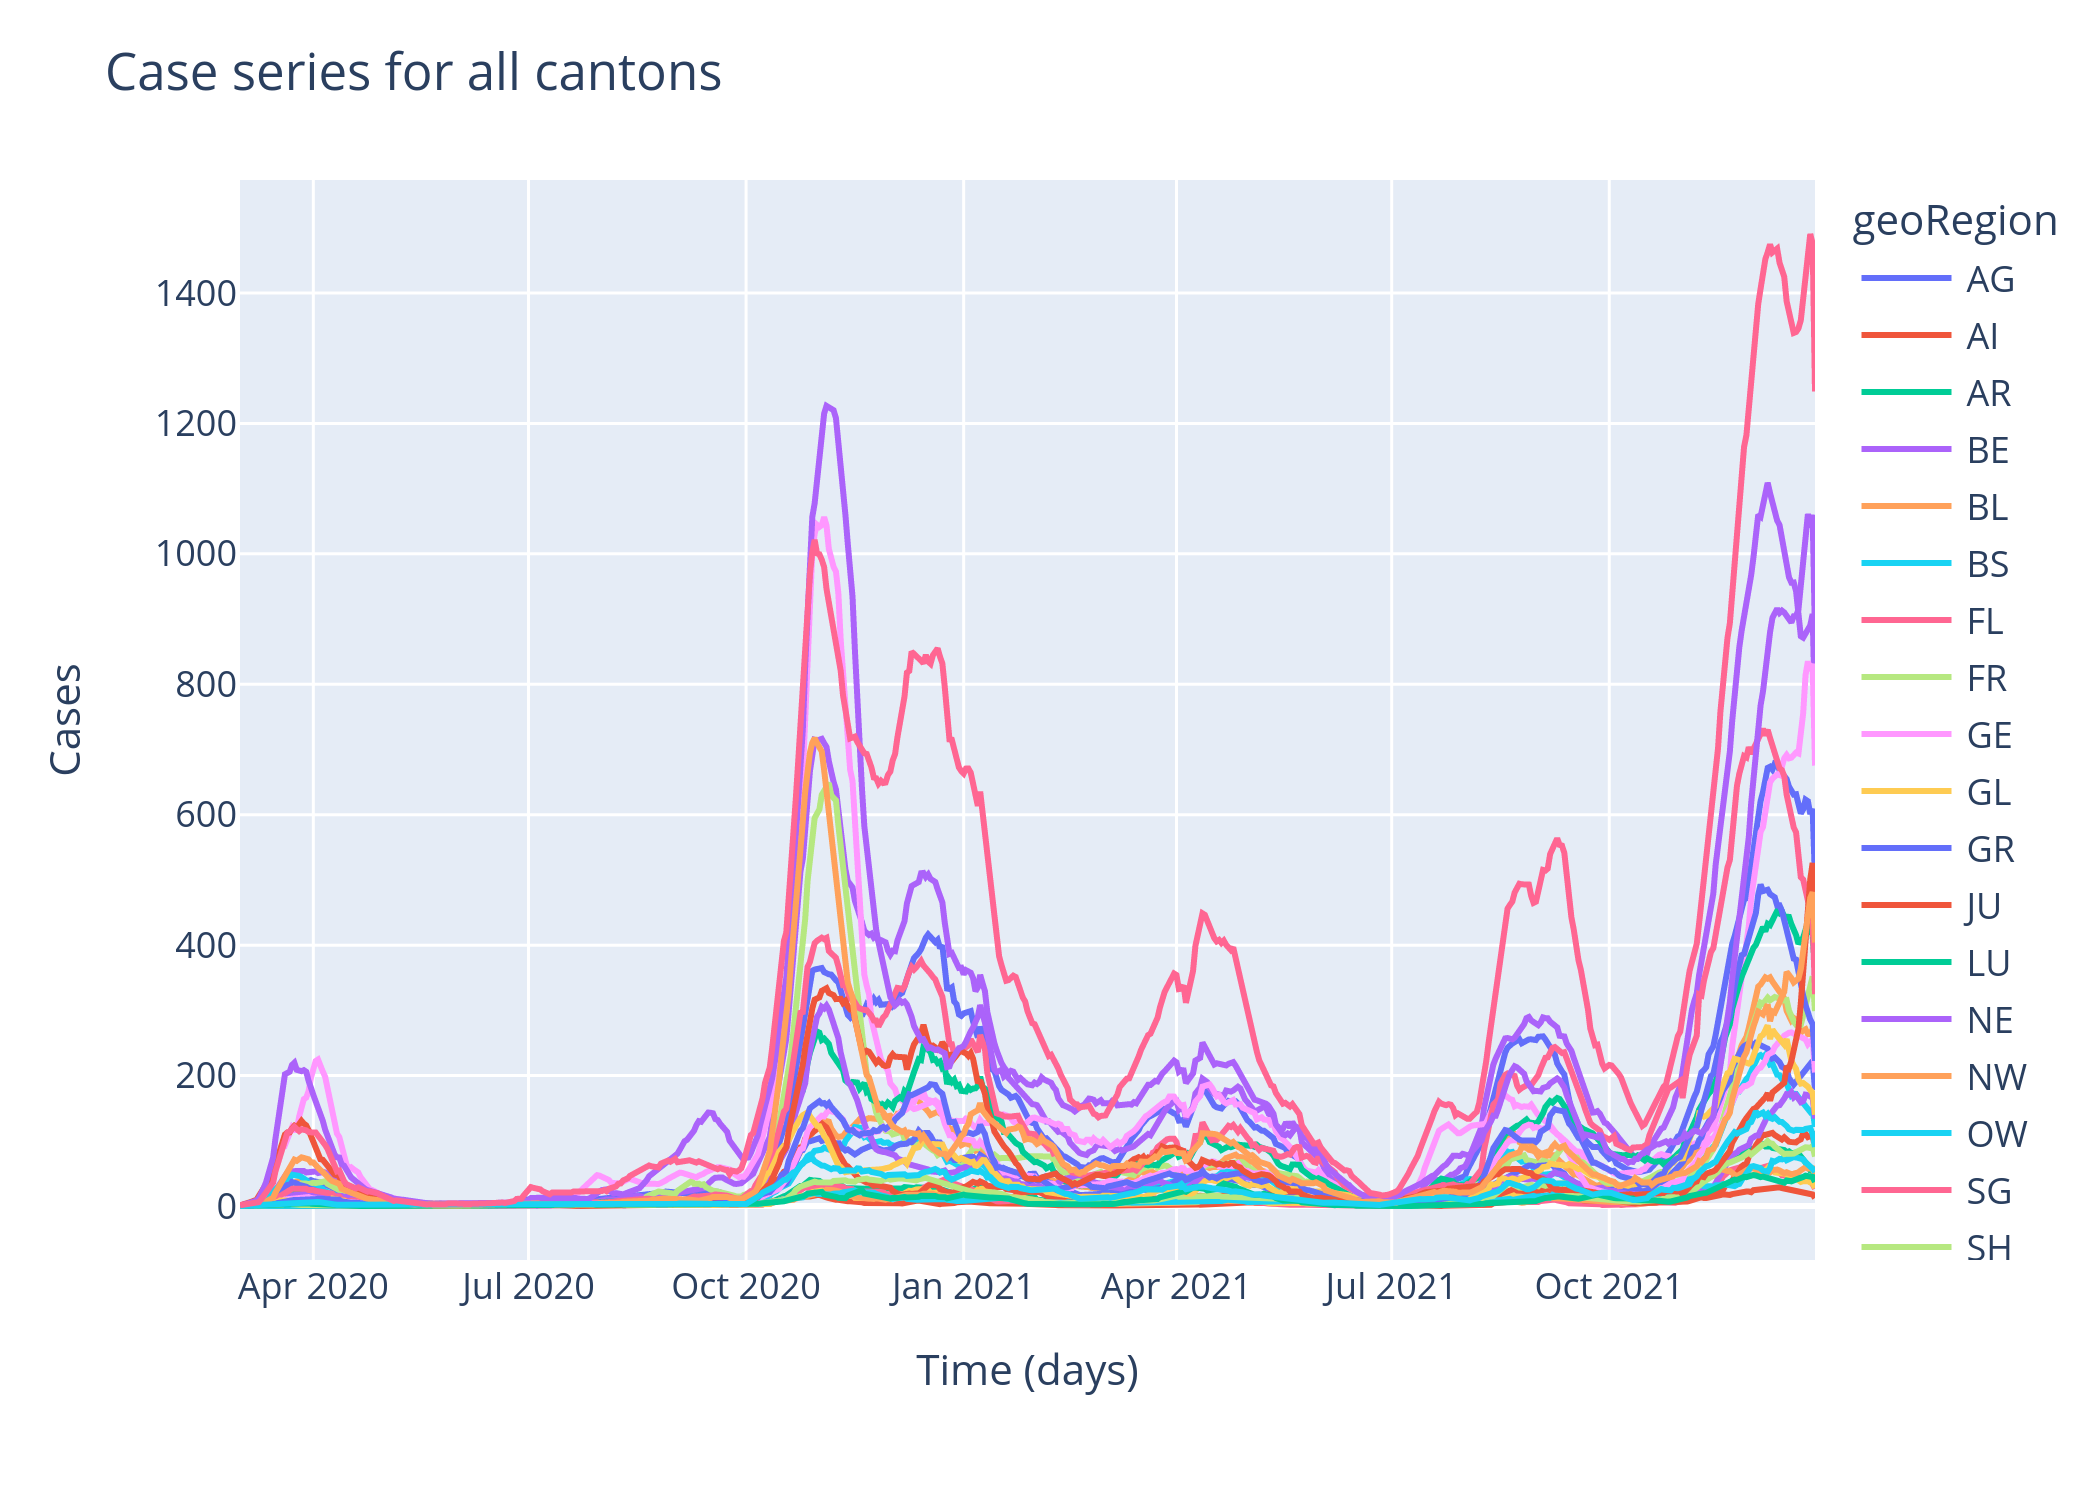
\includegraphics[width=\linewidth]{canton_series.png}
 % canton_series.png: 2100x1500 px, 72dpi, 74.08x52.92 cm, bb=0 0 2100 1500
 \caption{Timeseries of all cantons.}
 \label{fig:canton_series}
\end{figure}

    
    
    \hypertarget{calculating-the-cross-correlations}{%
\subsubsection{Calculating the
cross-correlations}\label{calculating-the-cross-correlations}}

If we take a closer look selected cantons we see that the most recent
wave started a little earlier on some cantons, relative to Geneva.
Notice that we also include the Vienna curve for reference.

\begin{figure}
 \centering
 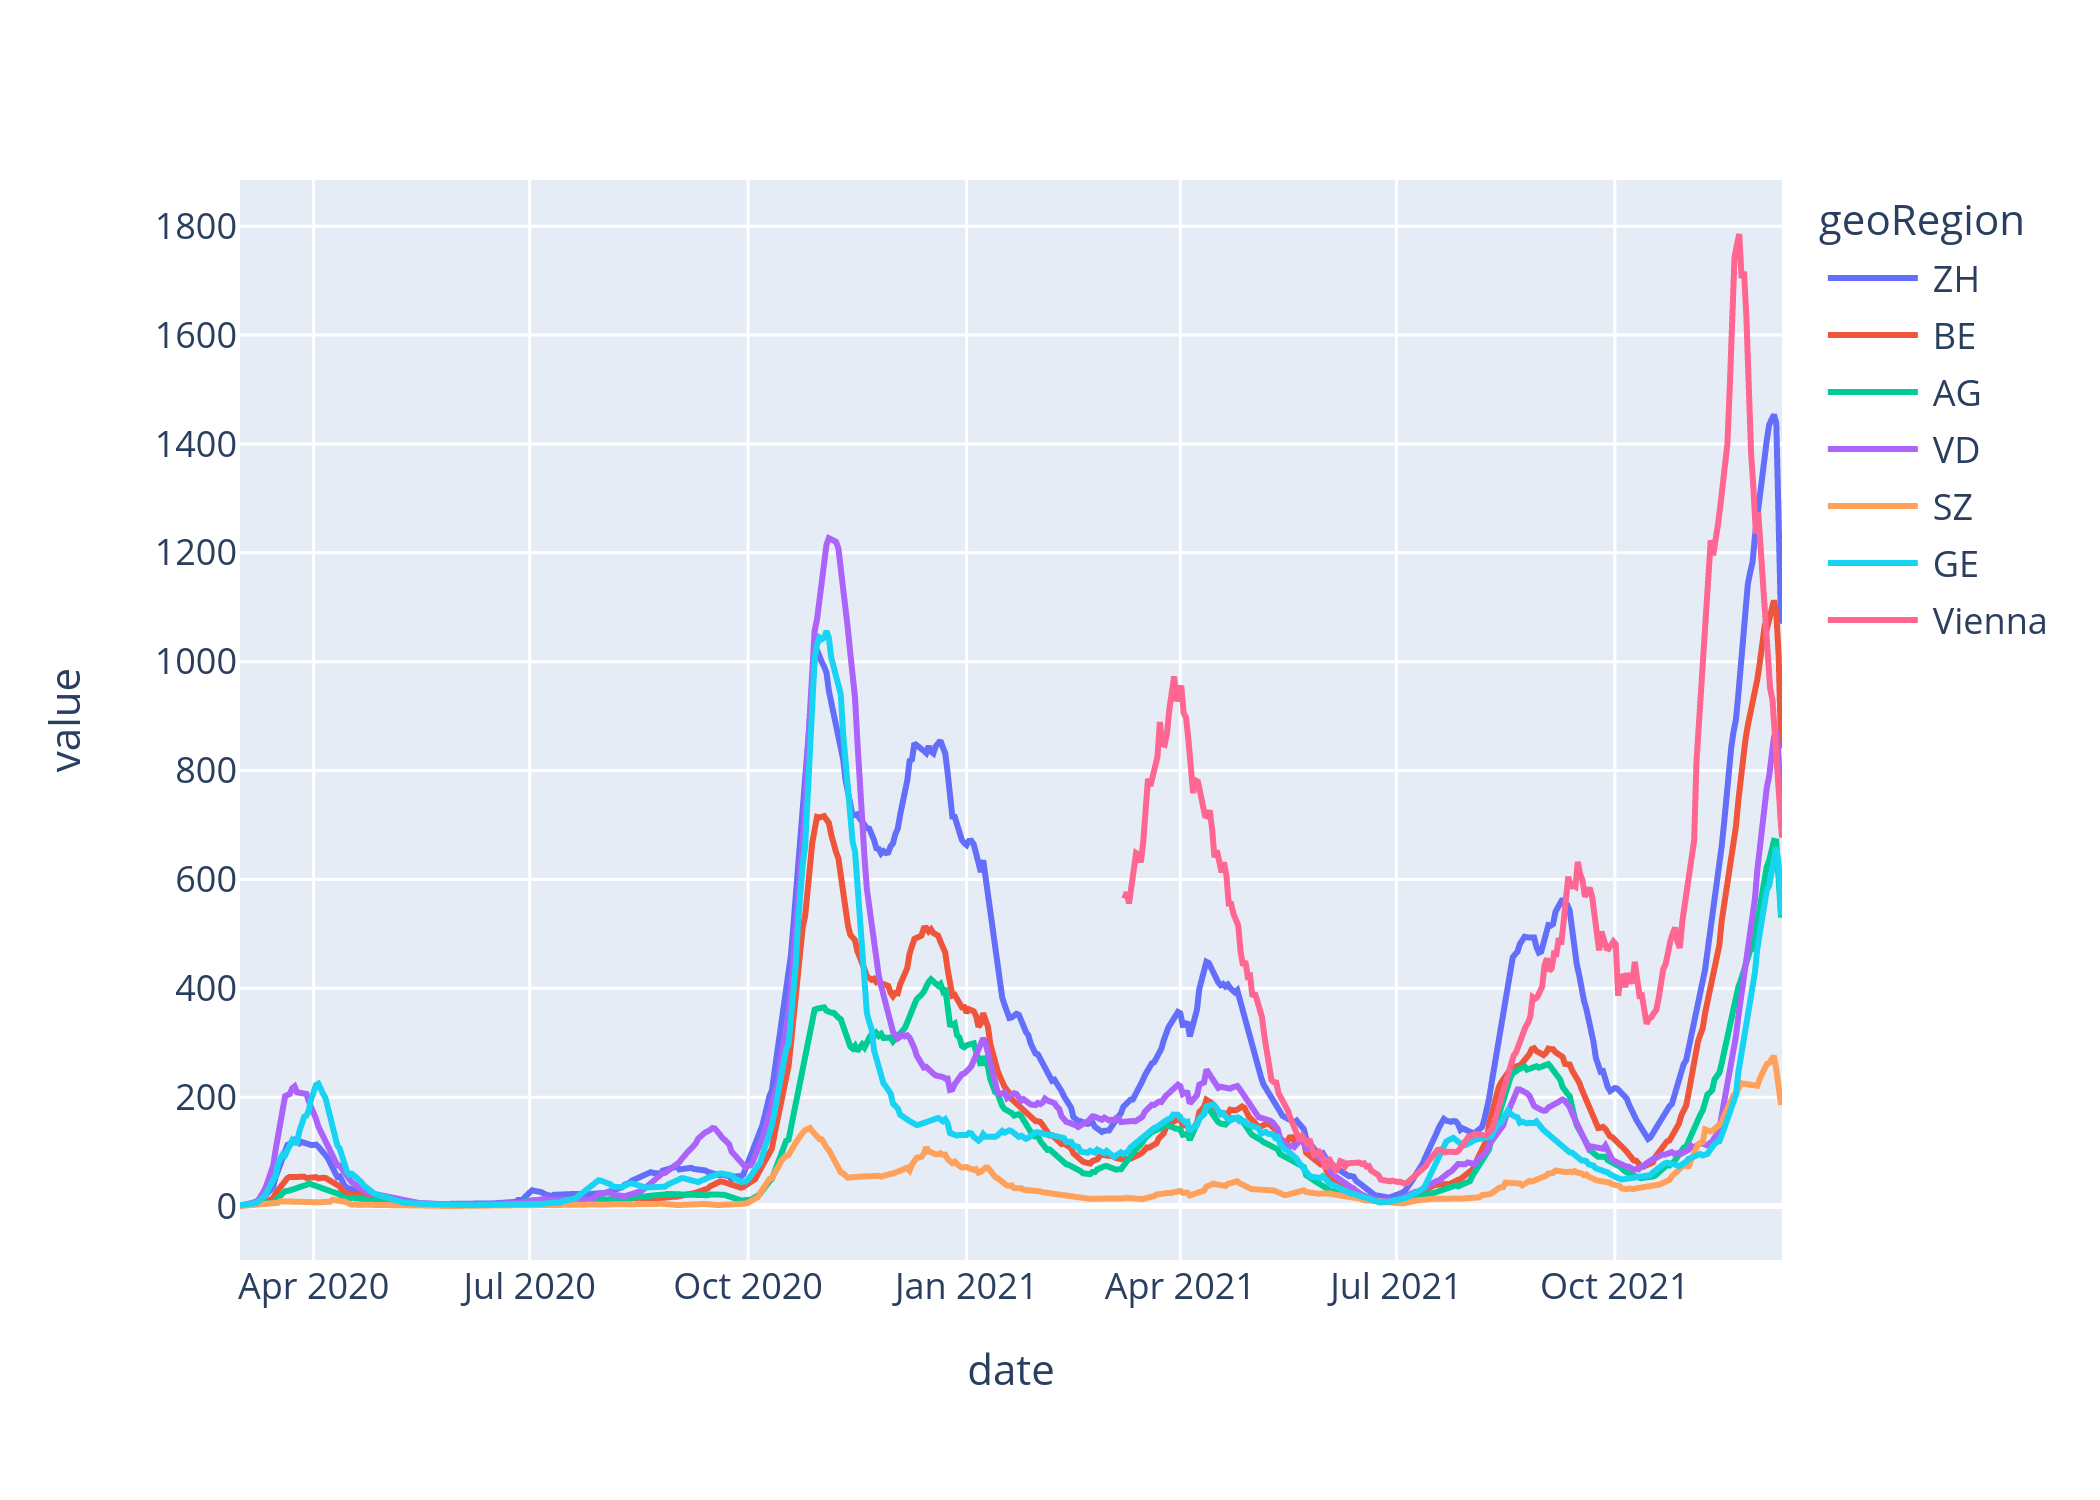
\includegraphics[width=\linewidth]{lagged_series.png}
 % lagged_series.png: 2100x1500 px, 72dpi, 74.08x52.92 cm, bb=0 0 2100 1500
 \caption{Selected swiss cantons and Vienna.}
 \label{fig:lagged series}
\end{figure}


    
    Looking at the cross correlation plot for some pairs of cantons, we can
see that the lag between them is not \(0\), which gives us hope that we
can use other series for predictive purposes.

    
    
    It's even better to look at all pairwise cross-correlations.

    
    
    
    
    \hypertarget{clustering-the-series-based-on-correlation}{%
\subsubsection{Clustering the Series based on
correlation}\label{clustering-the-series-based-on-correlation}}

    \begin{center}
    \adjustimage{max size={0.9\linewidth}{0.9\paperheight}}{Bayesian Hosp. rate_files/Bayesian Hosp. rate_64_0.png}
    \end{center}
    { \hspace*{\fill} \\}
    
    \hypertarget{geo-visualization}{%
\subsection{Geo visualization}\label{geo-visualization}}

    
    
    
    
    
    
            \begin{tcolorbox}[breakable, size=fbox, boxrule=.5pt, pad at break*=1mm, opacityfill=0]
\begin{Verbatim}[commandchars=\\\{\}]
   GID\_0       NAME\_0     GID\_1                  NAME\_1  \textbackslash{}
0    CHE  Switzerland   CHE.1\_1                  Aargau
1    CHE  Switzerland   CHE.2\_1  Appenzell Ausserrhoden
2    CHE  Switzerland   CHE.3\_1   Appenzell Innerrhoden
3    CHE  Switzerland   CHE.4\_1        Basel-Landschaft
4    CHE  Switzerland   CHE.5\_1             Basel-Stadt
5    CHE  Switzerland   CHE.6\_1                    Bern
6    CHE  Switzerland   CHE.7\_1                Fribourg
7    CHE  Switzerland   CHE.8\_1                  Genève
8    CHE  Switzerland   CHE.9\_1                  Glarus
9    CHE  Switzerland  CHE.10\_1              Graubünden
10   CHE  Switzerland  CHE.11\_1                    Jura
11   CHE  Switzerland  CHE.12\_1                 Lucerne
12   CHE  Switzerland  CHE.13\_1               Neuchâtel
13   CHE  Switzerland  CHE.14\_1               Nidwalden
14   CHE  Switzerland  CHE.15\_1                Obwalden
15   CHE  Switzerland  CHE.16\_1            Sankt Gallen
16   CHE  Switzerland  CHE.17\_1            Schaffhausen
17   CHE  Switzerland  CHE.18\_1                  Schwyz
18   CHE  Switzerland  CHE.19\_1               Solothurn
19   CHE  Switzerland  CHE.20\_1                 Thurgau
20   CHE  Switzerland  CHE.21\_1                  Ticino
21   CHE  Switzerland  CHE.22\_1                     Uri
22   CHE  Switzerland  CHE.23\_1                  Valais
23   CHE  Switzerland  CHE.24\_1                    Vaud
24   CHE  Switzerland  CHE.25\_1                     Zug
25   CHE  Switzerland  CHE.26\_1                  Zürich

                                            VARNAME\_1 NL\_NAME\_1  \textbackslash{}
0                             Argovia|Arg¢via|Argovie      None
1   Appenzell Ausser-Rhoden|Appenzell Outer Rhodes{\ldots}      None
2   Appenzell Inner-Rhoden|Appenzell Inner Rhodes|{\ldots}      None
3   Bâle-Campagne|Basel-Country|Baselland|Basel-La{\ldots}      None
4   Bâle-Ville|Basel-City|Basel-Town|Basilea-Citad{\ldots}      None
5                                         Berna|Berne      None
6                           Freiburg|Friburg|Friburgo      None
7   Cenevre|Genebra|Geneve|Geneva|Genevra|Genf|Gin{\ldots}      None
8                              Glaris|Glarona|Glaruna      None
9                Graubünden|Grigioni|Grischun|Grisons      None
10                                              Giura      None
11                                     Lucerna|Luzern      None
12                                          Neuenburg      None
13       Nidvaldo|Nidwald|Unterwalden-le-Bas|Nidwaldo      None
14  Obvaldo|Obwald|Unterwalden-le-Haut|Obwaldo|Sur{\ldots}      None
15                      Saint-Gall|San Gallo|Son Gagl      None
16                    Schaffhouse|Schaffusa|Sciaffusa      None
17                                               None      None
18                   Soletta|Soleure|Soleuro|Soloturn      None
19                        Thurgovie|Turgovia|Turg¢via      None
20                                      Tesino|Tessin      None
21                                               None      None
22                             Vallais|Vallese|Wallis      None
23                                Vad|Waadt|Waadtland      None
24                                          Zoug|Zugo      None
25                        Turitg|Zurigo|Zürih|Zurique      None

                   TYPE\_1 ENGTYPE\_1  CC\_1 HASC\_1  \textbackslash{}
0   Canton|Kanton|Chantun    Canton  None  CH.AG
1   Canton|Kanton|Chantun    Canton  None  CH.AR
2   Canton|Kanton|Chantun    Canton  None  CH.AI
3   Canton|Kanton|Chantun    Canton  None  CH.BL
4   Canton|Kanton|Chantun    Canton  None  CH.BS
5   Canton|Kanton|Chantun    Canton  None  CH.BE
6   Canton|Kanton|Chantun    Canton  None  CH.FR
7   Canton|Kanton|Chantun    Canton  None  CH.GE
8   Canton|Kanton|Chantun    Canton  None  CH.GL
9   Canton|Kanton|Chantun    Canton  None  CH.GR
10  Canton|Kanton|Chantun    Canton  None  CH.JU
11  Canton|Kanton|Chantun    Canton  None  CH.LU
12  Canton|Kanton|Chantun    Canton  None  CH.NE
13  Canton|Kanton|Chantun    Canton  None  CH.NW
14  Canton|Kanton|Chantun    Canton  None  CH.OW
15  Canton|Kanton|Chantun    Canton  None  CH.SG
16  Canton|Kanton|Chantun    Canton  None  CH.SH
17  Canton|Kanton|Chantun    Canton  None  CH.SZ
18  Canton|Kanton|Chantun    Canton  None  CH.SO
19  Canton|Kanton|Chantun    Canton  None  CH.TG
20  Canton|Kanton|Chantun    Canton  None  CH.TI
21  Canton|Kanton|Chantun    Canton  None  CH.UR
22  Canton|Kanton|Chantun    Canton  None  CH.VS
23  Canton|Kanton|Chantun    Canton  None  CH.VD
24  Canton|Kanton|Chantun    Canton  None  CH.ZG
25  Canton|Kanton|Chantun    Canton  None  CH.ZH

                                             geometry geoRegion  lags
0   MULTIPOLYGON (((7.94951 47.27751, 7.94897 47.2{\ldots}        AG   0.0
1   MULTIPOLYGON (((9.20708 47.27694, 9.20828 47.2{\ldots}        AR   0.0
2   MULTIPOLYGON (((9.51250 47.40100, 9.51430 47.4{\ldots}        AI   1.0
3   MULTIPOLYGON (((7.36526 47.41939, 7.36377 47.4{\ldots}        BL   0.0
4   MULTIPOLYGON (((7.55254 47.54676, 7.55290 47.5{\ldots}        BS   0.0
5   MULTIPOLYGON (((7.09284 46.89419, 7.09202 46.8{\ldots}        BE   0.0
6   MULTIPOLYGON (((6.78575 46.73603, 6.78559 46.7{\ldots}        FR   0.0
7   MULTIPOLYGON (((6.23440 46.33147, 6.23259 46.3{\ldots}        GE   0.0
8   MULTIPOLYGON (((8.90771 46.80860, 8.90603 46.8{\ldots}        GL   0.0
9   MULTIPOLYGON (((10.22766 46.61207, 10.22734 46{\ldots}        GR   0.0
10  MULTIPOLYGON (((6.97645 47.36205, 6.93670 47.3{\ldots}        JU   1.0
11  MULTIPOLYGON (((8.47390 47.12135, 8.47540 47.1{\ldots}        LU   0.0
12  MULTIPOLYGON (((6.46132 46.86218, 6.46295 46.8{\ldots}        NE   0.0
13  MULTIPOLYGON (((8.36748 46.78924, 8.36706 46.7{\ldots}        NW   0.0
14  MULTIPOLYGON (((8.39523 46.77334, 8.39626 46.7{\ldots}        OW   0.0
15  MULTIPOLYGON (((9.46901 46.90068, 9.46991 46.8{\ldots}        SG   0.0
16  MULTIPOLYGON (((8.85313 47.65377, 8.85196 47.6{\ldots}        SH   0.0
17  MULTIPOLYGON (((8.42042 47.06653, 8.41810 47.0{\ldots}        SZ   3.0
18  MULTIPOLYGON (((7.69325 47.15567, 7.68713 47.1{\ldots}        SO   0.0
19  MULTIPOLYGON (((9.18018 47.65754, 9.17886 47.6{\ldots}        TG   0.0
20  MULTIPOLYGON (((8.69525 46.10061, 8.69349 46.1{\ldots}        TI  -2.0
21  MULTIPOLYGON (((8.48248 46.52972, 8.48077 46.5{\ldots}        UR   0.0
22  MULTIPOLYGON (((7.61459 45.97337, 7.61351 45.9{\ldots}        VS   2.0
23  MULTIPOLYGON (((7.05791 46.86422, 7.05659 46.8{\ldots}        VD  -1.0
24  MULTIPOLYGON (((8.66821 47.16368, 8.67379 47.1{\ldots}        ZG   0.0
25  MULTIPOLYGON (((8.87364 47.24979, 8.86491 47.2{\ldots}        ZH   0.0
\end{Verbatim}
\end{tcolorbox}
        
    
    
            \begin{tcolorbox}[breakable, size=fbox, boxrule=.5pt, pad at break*=1mm, opacityfill=0]
\begin{Verbatim}[commandchars=\\\{\}]
:Polygons   [Longitude,Latitude]   (NAME\_1,geoRegion,lags)
\end{Verbatim}
\end{tcolorbox}
        
    \hypertarget{network-analysis}{%
\subsubsection{Network analysis}\label{network-analysis}}

We can take the correlation matrix and build a network to represent the
association between the cantons. for this network we will filter only
correlations greater than \(0.7\). We will use the correlation as the
weight of each edge.

    
    
    
    
    
    
            \begin{tcolorbox}[breakable, size=fbox, boxrule=.5pt, pad at break*=1mm, opacityfill=0]
\begin{Verbatim}[commandchars=\\\{\}]
AtlasView(\{0: \{'weight': 0.7813234254178534\}\})
\end{Verbatim}
\end{tcolorbox}
        
    \hypertarget{community-detection}{%
\paragraph{Community detection}\label{community-detection}}

The greedy moodularity algorithm detects two communities

    \begin{Verbatim}[commandchars=\\\{\}]
frozenset(\{'GR', 'GL', 'NW', 'SO', 'SG', 'TG', 'AR', 'OW', 'AI', 'LU', 'ZG',
'UR', 'SZ', 'SH', 'BL', 'BS'\})
frozenset(\{'VD', 'ZH', 'BE', 'NE', 'VS', 'AG', 'JU', 'FR', 'GE', 'TI'\})
    \end{Verbatim}

    
    
            \begin{tcolorbox}[breakable, size=fbox, boxrule=.5pt, pad at break*=1mm, opacityfill=0]
\begin{Verbatim}[commandchars=\\\{\}]
:Overlay
   .Graph.I  :Graph   [start,end]
   .Labels.I :Labels   [x,y]   (index)
\end{Verbatim}
\end{tcolorbox}
        
    \hypertarget{bayesian-inference}{%
\subsection{Bayesian Inference}\label{bayesian-inference}}

We would like to infer from the data some basic rates.

    We start by restricting our observations to 2021. So for the case series
we have:

            \begin{tcolorbox}[breakable, size=fbox, boxrule=.5pt, pad at break*=1mm, opacityfill=0]
\begin{Verbatim}[commandchars=\\\{\}]
           geoRegion       datum  entries  sumTotal  timeframe\_7d  \textbackslash{}
date
2021-01-01        GE  2021-01-01       64     44036         False
2021-01-02        GE  2021-01-02      126     44162         False
2021-01-03        GE  2021-01-03       72     44234         False
2021-01-04        GE  2021-01-04      153     44387         False
2021-01-05        GE  2021-01-05      163     44550         False
{\ldots}              {\ldots}         {\ldots}      {\ldots}       {\ldots}           {\ldots}
2021-11-27        GE  2021-11-27      330     80239          True
2021-11-28        GE  2021-11-28      227     80466          True
2021-11-29        GE  2021-11-29      742     81208          True
2021-11-30        GE  2021-11-30      442     81650          True
2021-12-01        GE  2021-12-01        0     81650         False

            offset\_last7d  sumTotal\_last7d  timeframe\_14d  offset\_last14d  \textbackslash{}
date
2021-01-01          78600                0          False           76706
2021-01-02          78600                0          False           76706
2021-01-03          78600                0          False           76706
2021-01-04          78600                0          False           76706
2021-01-05          78600                0          False           76706
{\ldots}                   {\ldots}              {\ldots}            {\ldots}             {\ldots}
2021-11-27          78600             1639           True           76706
2021-11-28          78600             1866           True           76706
2021-11-29          78600             2608           True           76706
2021-11-30          78600             3050           True           76706
2021-12-01          78600                0          False           76706

            sumTotal\_last14d  {\ldots}  inzsum14d  sumdelta7d  inzdelta7d  \textbackslash{}
date                          {\ldots}
2021-01-01                 0  {\ldots}     365.36        15.0        2.97
2021-01-02                 0  {\ldots}     367.54        28.0        5.52
2021-01-03                 0  {\ldots}     364.58        -8.0       -1.58
2021-01-04                 0  {\ldots}     354.11       -44.0       -8.68
2021-01-05                 0  {\ldots}     351.74       -21.0       -4.15
{\ldots}                      {\ldots}  {\ldots}        {\ldots}         {\ldots}         {\ldots}
2021-11-27              3533  {\ldots}     791.76       105.0       20.73
2021-11-28              3760  {\ldots}     824.14        93.0       18.37
2021-11-29              4502  {\ldots}     929.61       248.0       48.98
2021-11-30              4944  {\ldots}     976.41        60.0       11.85
2021-12-01                 0  {\ldots}     933.36      -423.0      -83.54

                    type  type\_variant              version  datum\_unit  \textbackslash{}
date
2021-01-01  COVID19Cases           NaN  2021-12-01\_07-53-57         day
2021-01-02  COVID19Cases           NaN  2021-12-01\_07-53-57         day
2021-01-03  COVID19Cases           NaN  2021-12-01\_07-53-57         day
2021-01-04  COVID19Cases           NaN  2021-12-01\_07-53-57         day
2021-01-05  COVID19Cases           NaN  2021-12-01\_07-53-57         day
{\ldots}                  {\ldots}           {\ldots}                  {\ldots}         {\ldots}
2021-11-27  COVID19Cases           NaN  2021-12-01\_07-53-57         day
2021-11-28  COVID19Cases           NaN  2021-12-01\_07-53-57         day
2021-11-29  COVID19Cases           NaN  2021-12-01\_07-53-57         day
2021-11-30  COVID19Cases           NaN  2021-12-01\_07-53-57         day
2021-12-01  COVID19Cases           NaN  2021-12-01\_07-53-57         day

            entries\_letzter\_stand  entries\_neu\_gemeldet  entries\_diff\_last
date
2021-01-01                     64                     0                818
2021-01-02                    126                     0                818
2021-01-03                     72                     0                818
2021-01-04                    153                     0                818
2021-01-05                    163                     0                818
{\ldots}                           {\ldots}                   {\ldots}                {\ldots}
2021-11-27                    328                     2                818
2021-11-28                    215                    12                818
2021-11-29                    364                   378                818
2021-11-30                      2                   440                818
2021-12-01                      0                     0                818

[335 rows x 57 columns]
\end{Verbatim}
\end{tcolorbox}
        
    For the Test series we have:

            \begin{tcolorbox}[breakable, size=fbox, boxrule=.5pt, pad at break*=1mm, opacityfill=0]
\begin{Verbatim}[commandchars=\\\{\}]
                 datum  entries  entries\_pos  entries\_neg  sumTotal  \textbackslash{}
date
2021-01-01  2021-01-01      581           66          515    291842
2021-01-02  2021-01-02     1178          125         1053    293020
2021-01-03  2021-01-03      663           75          588    293683
2021-01-04  2021-01-04     1961          157         1804    295644
2021-01-05  2021-01-05     2155          177         1978    297799
{\ldots}                {\ldots}      {\ldots}          {\ldots}          {\ldots}       {\ldots}
2021-11-26  2021-11-26     4672          551         4121   1025495
2021-11-27  2021-11-27     3092          459         2633   1028587
2021-11-28  2021-11-28     1392          264         1128   1029979
2021-11-29  2021-11-29     4342          664         3678   1034321
2021-11-30  2021-11-30     4355          689         3666   1038676

            timeframe\_7d  sumTotal\_last7d  timeframe\_14d  sumTotal\_last14d  \textbackslash{}
date
2021-01-01         False                0          False                 0
2021-01-02         False                0          False                 0
2021-01-03         False                0          False                 0
2021-01-04         False                0          False                 0
2021-01-05         False                0          False                 0
{\ldots}                  {\ldots}              {\ldots}            {\ldots}               {\ldots}
2021-11-26          True            12445           True             32565
2021-11-27          True            15537           True             35657
2021-11-28          True            16929           True             37049
2021-11-29          True            21271           True             41391
2021-11-30          True            25626           True             45746

            timeframe\_28d  {\ldots}  inzsumTotal\_Phase4  inzsum7d  inzsum14d  \textbackslash{}
date                       {\ldots}
2021-01-01          False  {\ldots}                <NA>   2094.63    5599.17
2021-01-02          False  {\ldots}                <NA>   2046.44    5485.02
2021-01-03          False  {\ldots}                <NA>   1998.84    5380.74
2021-01-04          False  {\ldots}                <NA>   1971.19    5103.26
2021-01-05          False  {\ldots}                <NA>   1992.13    4783.12
{\ldots}                   {\ldots}  {\ldots}                 {\ldots}       {\ldots}        {\ldots}
2021-11-26           True  {\ldots}            72227.72   4573.38    7990.83
2021-11-27           True  {\ldots}            72838.37   4714.59    8252.31
2021-11-28           True  {\ldots}            73113.28   4794.97    8357.77
2021-11-29           True  {\ldots}            73970.81   4973.11    8705.17
2021-11-30           True  {\ldots}             74830.9    5061.0    9034.59

                    type              version  datum\_unit  nachweismethode  \textbackslash{}
date
2021-01-01  COVID19Tests  2021-12-01\_07-53-57         day              all
2021-01-02  COVID19Tests  2021-12-01\_07-53-57         day              all
2021-01-03  COVID19Tests  2021-12-01\_07-53-57         day              all
2021-01-04  COVID19Tests  2021-12-01\_07-53-57         day              all
2021-01-05  COVID19Tests  2021-12-01\_07-53-57         day              all
{\ldots}                  {\ldots}                  {\ldots}         {\ldots}              {\ldots}
2021-11-26  COVID19Tests  2021-12-01\_07-53-57         day              all
2021-11-27  COVID19Tests  2021-12-01\_07-53-57         day              all
2021-11-28  COVID19Tests  2021-12-01\_07-53-57         day              all
2021-11-29  COVID19Tests  2021-12-01\_07-53-57         day              all
2021-11-30  COVID19Tests  2021-12-01\_07-53-57         day              all

            geoRegion  entries\_diff\_last\_age  entries\_diff\_last
date
2021-01-01         GE                      1               5660
2021-01-02         GE                      1               5660
2021-01-03         GE                      1               5660
2021-01-04         GE                      1               5660
2021-01-05         GE                      1               5660
{\ldots}               {\ldots}                    {\ldots}                {\ldots}
2021-11-26         GE                      1               5660
2021-11-27         GE                      1               5660
2021-11-28         GE                      1               5660
2021-11-29         GE                      1               5660
2021-11-30         GE                      1               5660

[334 rows x 54 columns]
\end{Verbatim}
\end{tcolorbox}
        
    And finally, the hospitalization series become:

            \begin{tcolorbox}[breakable, size=fbox, boxrule=.5pt, pad at break*=1mm, opacityfill=0]
\begin{Verbatim}[commandchars=\\\{\}]
           geoRegion       datum  entries  sumTotal  timeframe\_7d  \textbackslash{}
date
2021-01-01        GE  2021-01-01        6      1022         False
2021-01-02        GE  2021-01-02        4      1026         False
2021-01-03        GE  2021-01-03        5      1031         False
2021-01-04        GE  2021-01-04        5      1036         False
2021-01-05        GE  2021-01-05        2      1038         False
{\ldots}              {\ldots}         {\ldots}      {\ldots}       {\ldots}           {\ldots}
2021-11-27        GE  2021-11-27        0      2021          True
2021-11-28        GE  2021-11-28        0      2021          True
2021-11-29        GE  2021-11-29        0      2021          True
2021-11-30        GE  2021-11-30        0      2021          True
2021-12-01        GE  2021-12-01        0      2021         False

            offset\_last7d  sumTotal\_last7d  timeframe\_14d  offset\_last14d  \textbackslash{}
date
2021-01-01           2021                0          False            2019
2021-01-02           2021                0          False            2019
2021-01-03           2021                0          False            2019
2021-01-04           2021                0          False            2019
2021-01-05           2021                0          False            2019
{\ldots}                   {\ldots}              {\ldots}            {\ldots}             {\ldots}
2021-11-27           2021                0           True            2019
2021-11-28           2021                0           True            2019
2021-11-29           2021                0           True            2019
2021-11-30           2021                0           True            2019
2021-12-01           2021                0          False            2019

            sumTotal\_last14d  {\ldots}  inzsum14d  sumdelta7d  inzdelta7d  \textbackslash{}
date                          {\ldots}
2021-01-01                 0  {\ldots}      10.66         1.0        0.20
2021-01-02                 0  {\ldots}      11.06         3.0        0.59
2021-01-03                 0  {\ldots}      11.45         1.0        0.20
2021-01-04                 0  {\ldots}      11.85        -1.0       -0.20
2021-01-05                 0  {\ldots}      11.85        -2.0       -0.40
{\ldots}                      {\ldots}  {\ldots}        {\ldots}         {\ldots}         {\ldots}
2021-11-27                 2  {\ldots}       0.39         0.0        0.00
2021-11-28                 2  {\ldots}       0.39        -1.0       -0.20
2021-11-29                 2  {\ldots}       0.39         0.0        0.00
2021-11-30                 2  {\ldots}       0.39         0.0        0.00
2021-12-01                 0  {\ldots}       0.39         0.0        0.00

                   type  type\_variant              version  datum\_unit  \textbackslash{}
date
2021-01-01  COVID19Hosp           NaN  2021-12-01\_07-53-57         day
2021-01-02  COVID19Hosp           NaN  2021-12-01\_07-53-57         day
2021-01-03  COVID19Hosp           NaN  2021-12-01\_07-53-57         day
2021-01-04  COVID19Hosp           NaN  2021-12-01\_07-53-57         day
2021-01-05  COVID19Hosp           NaN  2021-12-01\_07-53-57         day
{\ldots}                 {\ldots}           {\ldots}                  {\ldots}         {\ldots}
2021-11-27  COVID19Hosp           NaN  2021-12-01\_07-53-57         day
2021-11-28  COVID19Hosp           NaN  2021-12-01\_07-53-57         day
2021-11-29  COVID19Hosp           NaN  2021-12-01\_07-53-57         day
2021-11-30  COVID19Hosp           NaN  2021-12-01\_07-53-57         day
2021-12-01  COVID19Hosp           NaN  2021-12-01\_07-53-57         day

            entries\_letzter\_stand  entries\_neu\_gemeldet  entries\_diff\_last
date
2021-01-01                      6                     0                  0
2021-01-02                      4                     0                  0
2021-01-03                      5                     0                  0
2021-01-04                      5                     0                  0
2021-01-05                      2                     0                  0
{\ldots}                           {\ldots}                   {\ldots}                {\ldots}
2021-11-27                      0                     0                  0
2021-11-28                      0                     0                  0
2021-11-29                      0                     0                  0
2021-11-30                      0                     0                  0
2021-12-01                      0                     0                  0

[335 rows x 57 columns]
\end{Verbatim}
\end{tcolorbox}
        
    \hypertarget{cases-and-hospitalizations-as-binomial-processes-with-variable-rates}{%
\subsubsection{Cases and Hospitalizations as Binomial processes with
variable
rates}\label{cases-and-hospitalizations-as-binomial-processes-with-variable-rates}}

If we treat cases and hospitalizations as bionomial processes, we can
estimate their variable rates. From the Test series, \(T_t\) we can
model the prevalence series in the population,
\(Pv_t \sim Beta (\alpha, \beta)\) as

\[Cases_t \sim Bin(n=T_t, p=Pv_t).\]

In a similar fashion, we can model the probability of Hospitalization,
\(Ph_t \sim Beta (\alpha, \beta)\) as

\[Hospitalizations_t \sim Bin(n=Cases_t, p=Ph_t).\]

    \begin{Verbatim}[commandchars=\\\{\}]
Auto-assigning NUTS sampler{\ldots}
Initializing NUTS using jitter+adapt\_diag{\ldots}
Multiprocess sampling (4 chains in 4 jobs)
NUTS: [Phosp, Prevalence]
    \end{Verbatim}

    
    \begin{Verbatim}[commandchars=\\\{\}]
<IPython.core.display.HTML object>
    \end{Verbatim}

    
    \begin{Verbatim}[commandchars=\\\{\}]
Sampling 4 chains for 1\_000 tune and 1\_000 draw iterations (4\_000 + 4\_000 draws
total) took 26 seconds.
    \end{Verbatim}

    The diagram of our inference becomes:
 
            
    
    \begin{center}
    \adjustimage{max size={0.9\linewidth}{0.9\paperheight}}{Bayesian Hosp. rate_files/Bayesian Hosp. rate_95_0.pdf}
    \end{center}
    { \hspace*{\fill} \\}
    

    Which after our estimation yields the following probability distribution
over time for the prevalence. Notice that it matches quite well the test
positivity data (purple dots).

    
    
    
    
    \hypertarget{sir-based-forecasting}{%
\subsubsection{SIR-based Forecasting}\label{sir-based-forecasting}}

The FOPH makes available the daily estimates of the effective
reproductive number, \(R_t\). With a goo estimate of R\_t it is possible
to simulate growth based on transmission models. Since for the SIR
model, \[R_t = R_0 S(t)= \frac{\beta}{\gamma}S(t),\] we can use it to
parameterize a simple transmission model with which to forcast cases and
thus hospitalizations. We would normally write the SIR model as:

\begin{align}
\frac{dS}{dt} &= -\beta S(t)I(t)\\
\frac{dI}{dt} &= \beta S(t)I(t) -\gamma I(t)
\end{align}

From the \(R_t\) time series, we can derive a time-dependent
transmission parameter, \[\beta(t)=\frac{R_t \gamma}{S(t)}.\]

Then we can re-write the SIR model as

\begin{align}
\frac{dS}{dt} &= -R_t\gamma I(t)\\
\frac{dI}{dt} &= R_t\gamma I(t) -\gamma I(t) \label{eq:I}
\end{align}

We can reduce the system above to just equation \ref{eq:I}, which has
the following solution:

\[I(t) = I(0) e^{(R_t-1)\gamma t}\]

The \emph{prevalence} in the population that we estimated before, in the
SIR model is given by \(I(t)\). We can see that its evolution is
dependent of the effective reproductive number, and our ability to
forecast it. We can also easily propagate the uncertainty of the \(R_t\)
estimate to obtain uncertainty bands for I(t) as well.

    Let's apply this inference just to the last wave starting on october,
15th. To facilitate the fit to the model let's also use the 7-day moving
average of it.

    
    
            \begin{tcolorbox}[breakable, size=fbox, boxrule=.5pt, pad at break*=1mm, opacityfill=0]
\begin{Verbatim}[commandchars=\\\{\}]
date
2021-10-14    1.12
2021-10-15    1.10
2021-10-16    1.07
2021-10-17    1.05
2021-10-18    1.04
2021-10-19    1.03
2021-10-20    1.03
2021-10-21    1.04
2021-10-22    1.06
2021-10-23    1.07
2021-10-24    1.09
2021-10-25    1.09
2021-10-26    1.10
2021-10-27    1.10
2021-10-28    1.10
2021-10-29    1.11
2021-10-30    1.12
2021-10-31    1.13
2021-11-01    1.13
2021-11-02    1.13
2021-11-03    1.14
2021-11-04    1.17
2021-11-05    1.22
2021-11-06    1.27
2021-11-07    1.33
2021-11-08    1.39
2021-11-09    1.45
2021-11-10    1.51
2021-11-11    1.57
2021-11-12    1.61
2021-11-13    1.63
2021-11-14    1.62
2021-11-15    1.59
2021-11-16     NaN
2021-11-17     NaN
2021-11-18     NaN
2021-11-19     NaN
2021-11-20     NaN
2021-11-21     NaN
2021-11-22     NaN
2021-11-23     NaN
2021-11-24     NaN
2021-11-25     NaN
2021-11-26     NaN
2021-11-27     NaN
2021-11-28     NaN
2021-11-29     NaN
2021-11-30     NaN
2021-12-01     NaN
Name: median\_R\_mean, dtype: float64
\end{Verbatim}
\end{tcolorbox}
        
    The structure of the probabilistic model is depicted below.
 
            
    
    \begin{center}
    \adjustimage{max size={0.9\linewidth}{0.9\paperheight}}{Bayesian Hosp. rate_files/Bayesian Hosp. rate_106_0.pdf}
    \end{center}
    { \hspace*{\fill} \\}
    

    \begin{Verbatim}[commandchars=\\\{\}]
Auto-assigning NUTS sampler{\ldots}
Initializing NUTS using jitter+adapt\_diag{\ldots}
Multiprocess sampling (4 chains in 4 jobs)
NUTS: [I0, gamma, sigma]
    \end{Verbatim}

    
    \begin{Verbatim}[commandchars=\\\{\}]
<IPython.core.display.HTML object>
    \end{Verbatim}

    
    \begin{Verbatim}[commandchars=\\\{\}]
Sampling 4 chains for 1\_900 tune and 2\_000 draw iterations (7\_600 + 8\_000 draws
total) took 8 seconds.
There was 1 divergence after tuning. Increase `target\_accept` or reparameterize.
The acceptance probability does not match the target. It is 0.884699057698102,
but should be close to 0.8. Try to increase the number of tuning steps.
    \end{Verbatim}

            \begin{tcolorbox}[breakable, size=fbox, boxrule=.5pt, pad at break*=1mm, opacityfill=0]
\begin{Verbatim}[commandchars=\\\{\}]
Inference data with groups:
        > posterior
        > log\_likelihood
        > sample\_stats
        > observed\_data
\end{Verbatim}
\end{tcolorbox}
        
    \begin{center}
    \adjustimage{max size={0.9\linewidth}{0.9\paperheight}}{Bayesian Hosp. rate_files/Bayesian Hosp. rate_109_0.png}
    \end{center}
    { \hspace*{\fill} \\}
    
    
    
    \hypertarget{forecasting}{%
\subsection{Forecasting}\label{forecasting}}

We applied Machine-learning approaches to Forecasting, namely KNN and
LightGBM.

\begin{figure}
\centering
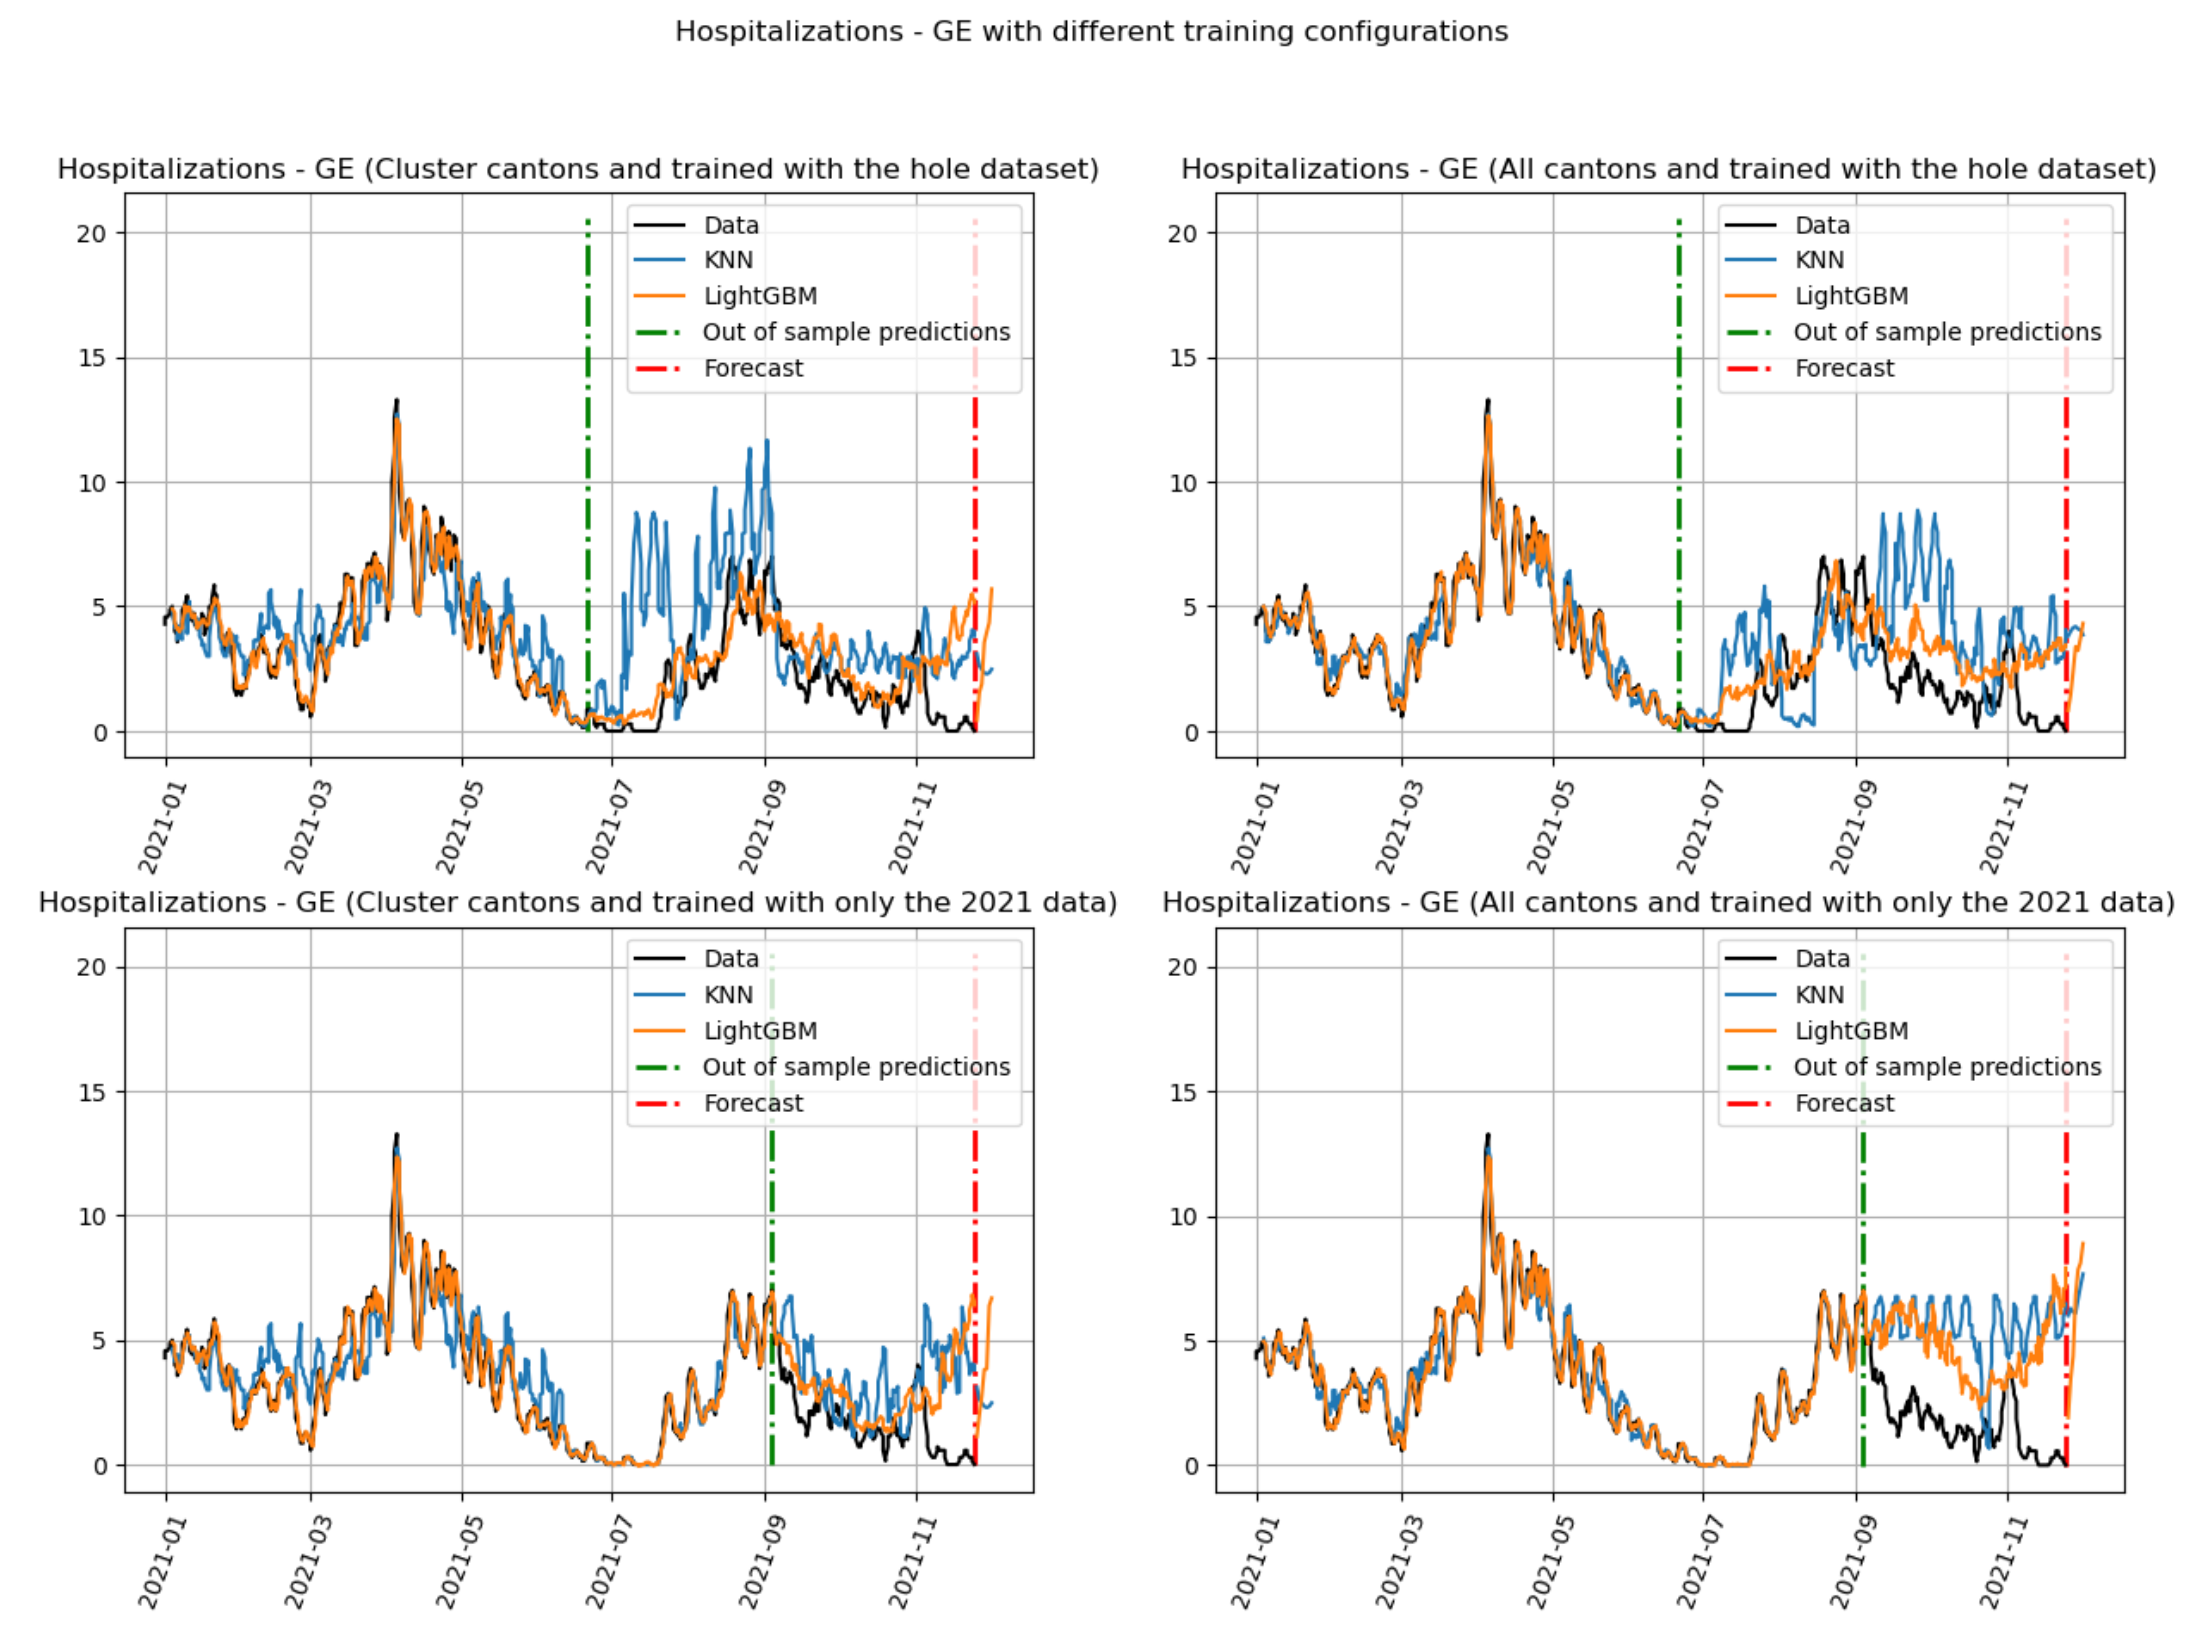
\includegraphics{forecasts.png}
\caption{forecasts}
\end{figure}

    \hypertarget{lightgbm-model}{%
\subsubsection{Lightgbm model}\label{lightgbm-model}}

    
    \begin{Verbatim}[commandchars=\\\{\}]
<IPython.core.display.HTML object>
    \end{Verbatim}

    
    \begin{Verbatim}[commandchars=\\\{\}]
The watermark extension is already loaded. To reload it, use:
  \%reload\_ext watermark
Last updated: Fri Nov 26 2021

Python implementation: CPython
Python version       : 3.9.7
IPython version      : 7.28.0

requests  : 2.25.1
seaborn   : 0.11.2
json      : 2.0.9
numpy     : 1.20.3
plotly    : 5.4.0
matplotlib: 3.5.0
lightgbm  : 3.3.1
pandas    : 1.3.4

Watermark: 2.2.0

    \end{Verbatim}

            \begin{tcolorbox}[breakable, size=fbox, boxrule=.5pt, pad at break*=1mm, opacityfill=0]
\begin{Verbatim}[commandchars=\\\{\}]
(642, 27)
\end{Verbatim}
\end{tcolorbox}
        

    % Add a bibliography block to the postdoc
    
    
    
\end{document}
